% !Mode:: "TeX:UTF-8"

\chapter{前端页面展示}

本项目前端基于Vue.js 3框架和Element Plus组件库构建，采用单页面应用（SPA）架构，实现了响应式布局和组件化开发。以下按功能模块展示各核心页面。

\section{用户认证模块}

\subsection{登录页面}

\begin{figure}[H]
	\centering
	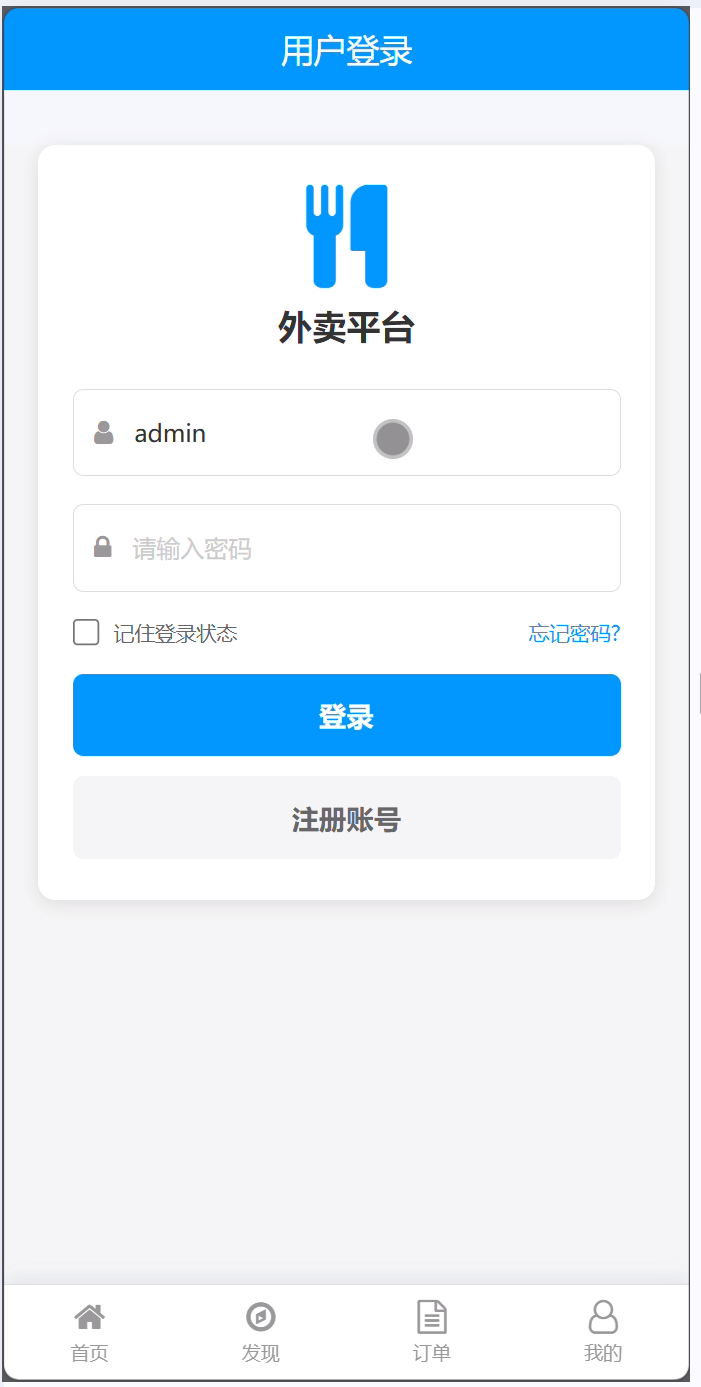
\includegraphics[width=0.75\textwidth,height=0.82\textheight,keepaspectratio]{images/page-login.png}
	\caption{登录页面}
	\label{fig:login-page}
\end{figure}

登录页面（Login.vue）提供用户名和密码输入表单，支持表单验证（必填项检查）。用户提交登录请求后，前端调用\verb|POST /api/auth|获取JWT Token，将Token存入localStorage并跳转至首页。页面顶部展示项目Logo和标题"ELM外卖平台"，底部提供"去注册"的导航链接。

\subsection{注册页面}

\begin{figure}[H]
	\centering
	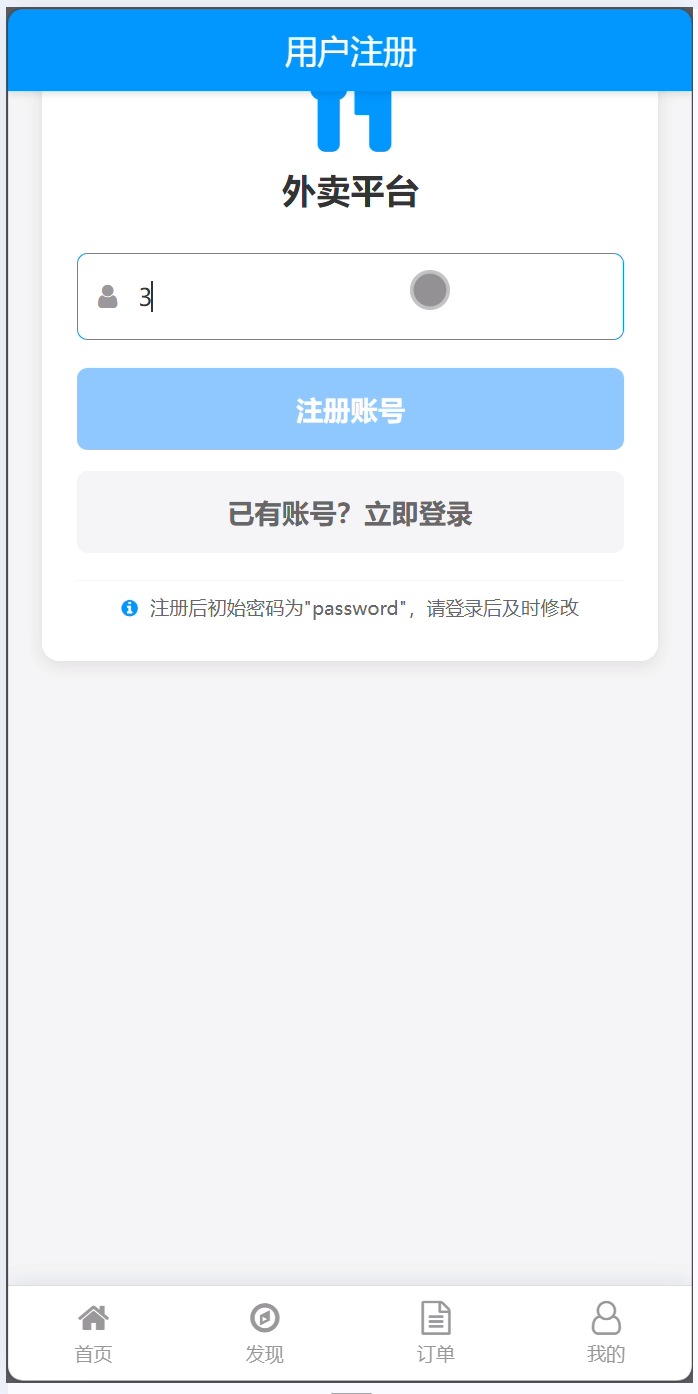
\includegraphics[width=0.75\textwidth,height=0.82\textheight,keepaspectratio]{images/page-register.png}
	\caption{注册页面}
	\label{fig:register-page}
\end{figure}

注册页面（Register.vue）提供用户名、密码、确认密码、用户性别等注册信息表单。前端对密码和确认密码进行一致性校验，对用户名长度进行合法性检查。提交注册请求至\verb|POST /api/register|，注册成功后自动跳转至登录页面。


\section{首页与导航}

\subsection{首页}

\begin{figure}[H]
	\centering
	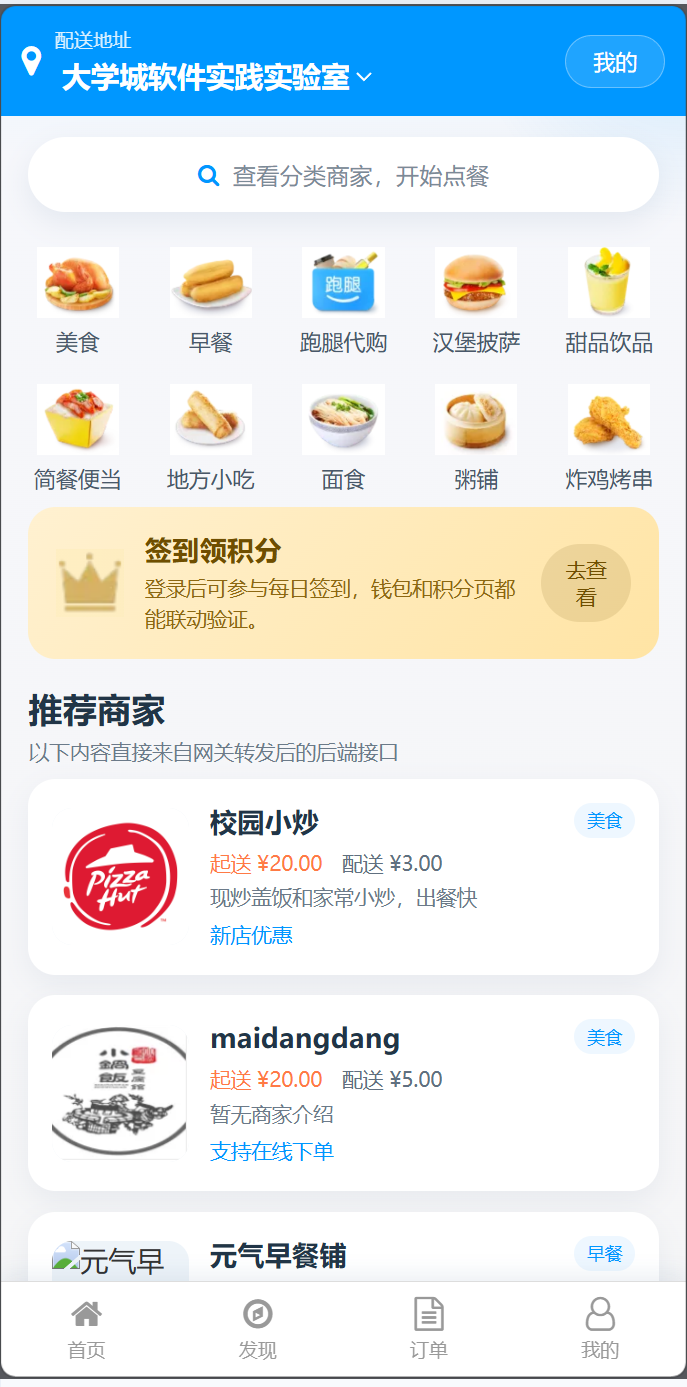
\includegraphics[width=0.75\textwidth,height=0.82\textheight,keepaspectratio]{images/page-index.png}
	\caption{首页}
	\label{fig:index-page}
\end{figure}

首页（Index.vue）作为用户登录后的主入口，展示顶部导航栏（包含商家列表、订单、购物车、钱包、积分等入口），中间区域展示轮播Banner和推荐商家列表，底部展示版权信息。导航栏根据用户登录状态动态显示不同菜单项。

\subsection{用户首页}

\begin{figure}[H]
	\centering
	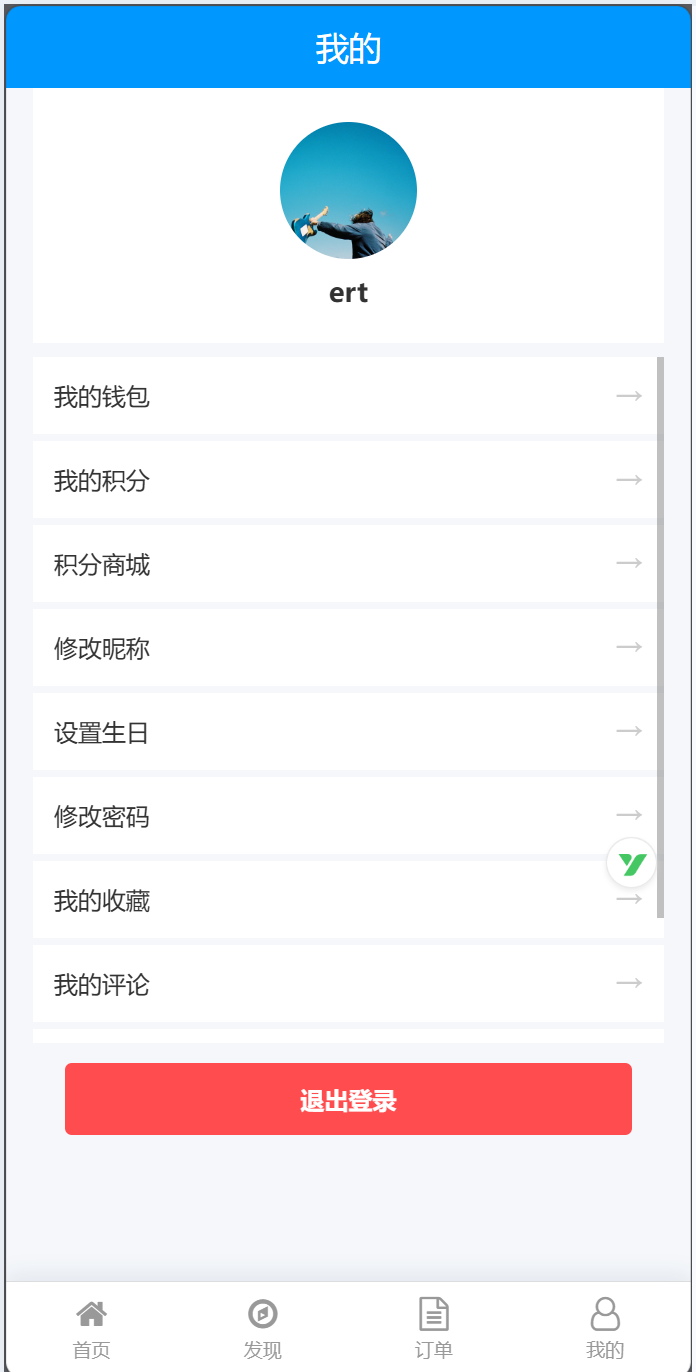
\includegraphics[width=0.75\textwidth,height=0.82\textheight,keepaspectratio]{images/page-user-home.png}
	\caption{用户首页}
	\label{fig:user-home-page}
\end{figure}

用户首页（UserHome.vue）展示用户个人信息概览，包括用户名、头像、会员等级，以及快捷入口卡片（我的订单、钱包余额、可用积分、VIP状态等）。

\section{商家模块}

\subsection{商家列表页面}

\begin{figure}[H]
	\centering
	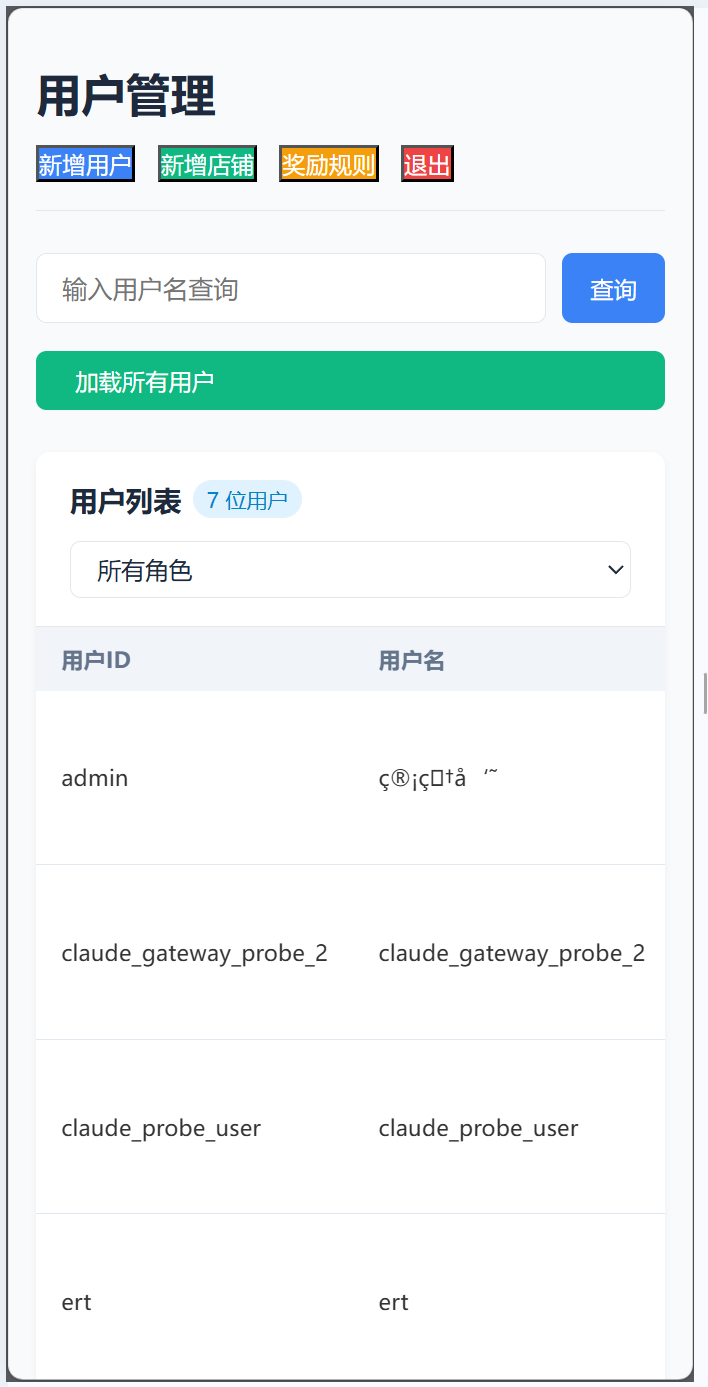
\includegraphics[width=0.75\textwidth,height=0.82\textheight,keepaspectratio]{images/page-business-list.png}
	\caption{商家列表页面}
	\label{fig:business-list-page}
\end{figure}

商家列表页面（BusinessList.vue）以卡片列表形式展示所有注册商家，每张卡片包含商家名称、商家图片、起送价（starPrice）、配送费（deliveryPrice）、商家简介和评分信息。支持按商家名称搜索和按配送费/起送价排序。点击商家卡片进入商家详情页。

\subsection{商家详情页面}

\begin{figure}[H]
	\centering
	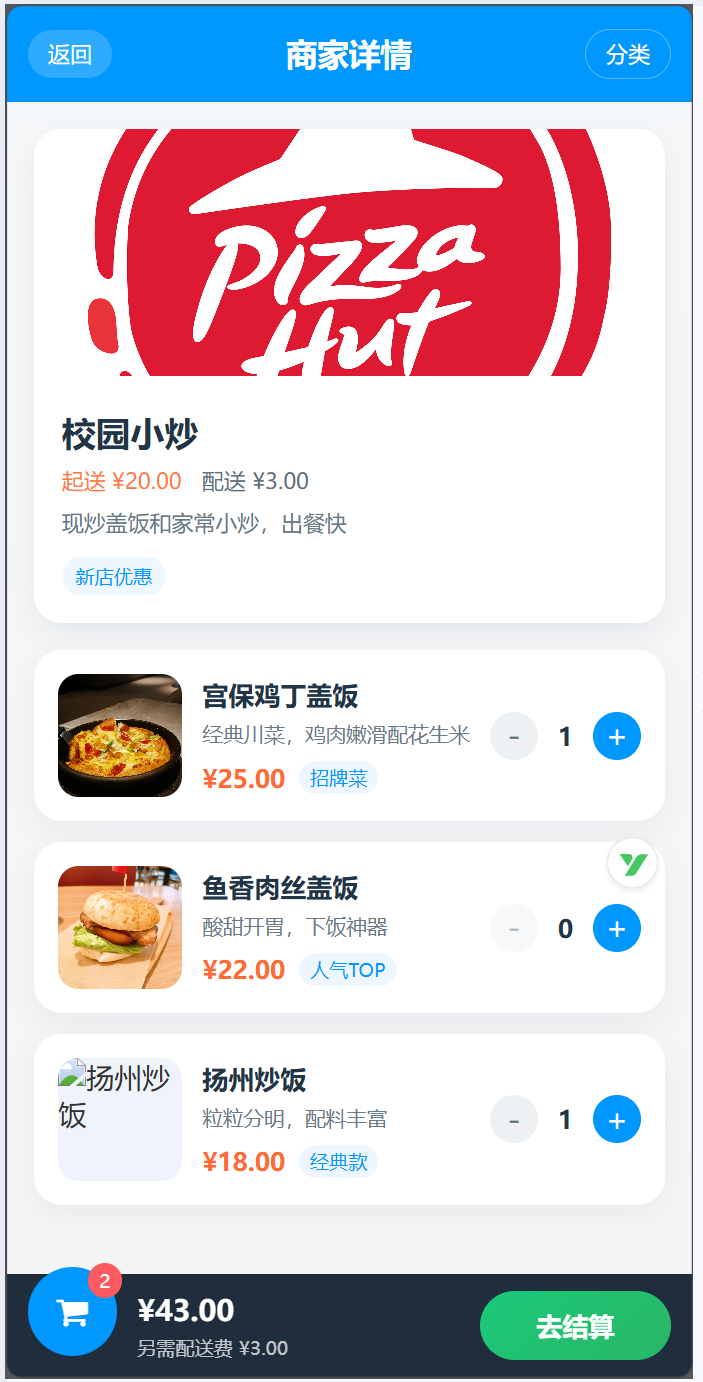
\includegraphics[width=0.75\textwidth,height=0.82\textheight,keepaspectratio]{images/page-business-info.png}
	\caption{商家详情页面}
	\label{fig:business-info-page}
\end{figure}

商家详情页面（BusinessInfo.vue）展示单个商家的完整信息，包括商家头图、名称、地址、简介、营业时间和备注。页面下方以列表形式展示该商家所有在售食品，每项食品显示名称、图片、价格（元）和简介，支持"加入购物车"按钮。食品列表通过\verb|GET /foods?businessId={id}|获取。

\subsection{商家管理页面}

\begin{figure}[H]
	\centering
	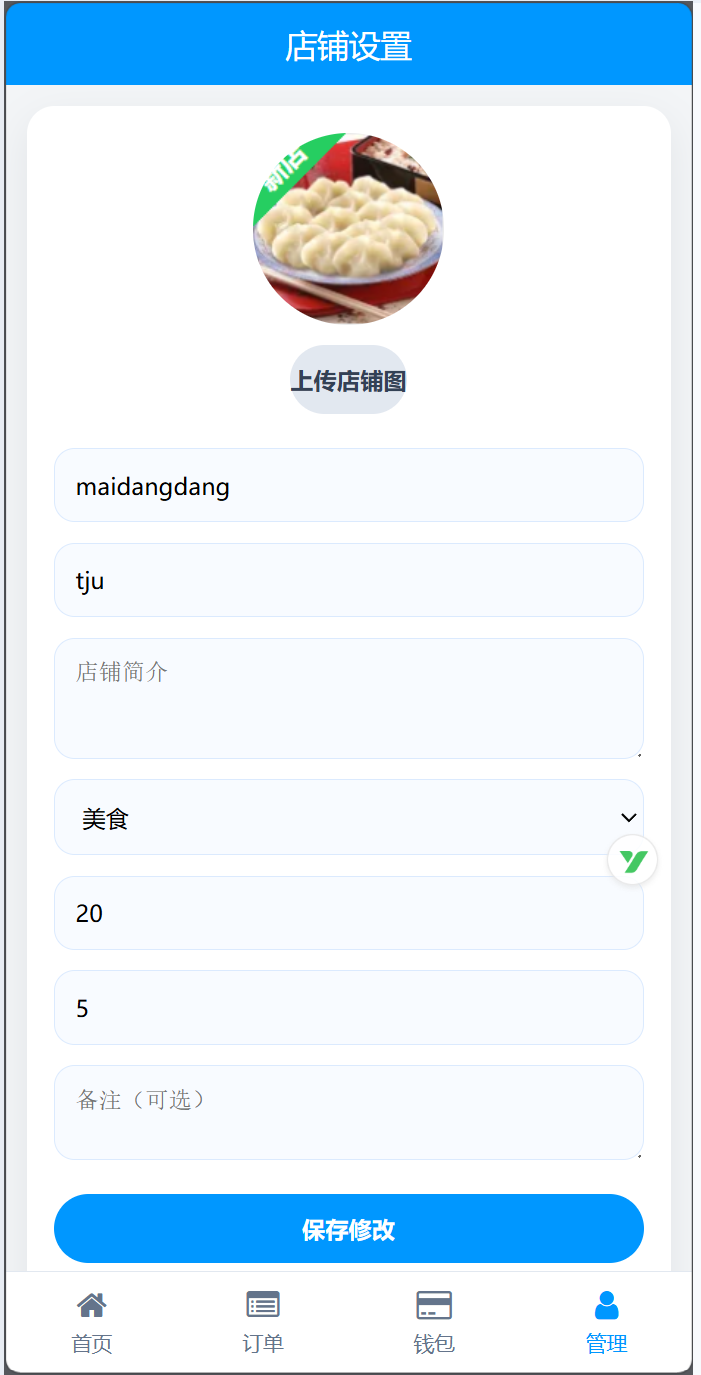
\includegraphics[width=0.75\textwidth,height=0.82\textheight,keepaspectratio]{images/page-business-manage.png}
	\caption{商家管理页面}
	\label{fig:business-manage-page}
\end{figure}

商家管理页面（BusinessManage.vue）展示当前用户拥有的商家列表，支持编辑商家信息。商家所有者可以查看该商家收到的订单列表。

\subsection{商家订单页面}

\begin{figure}[H]
	\centering
	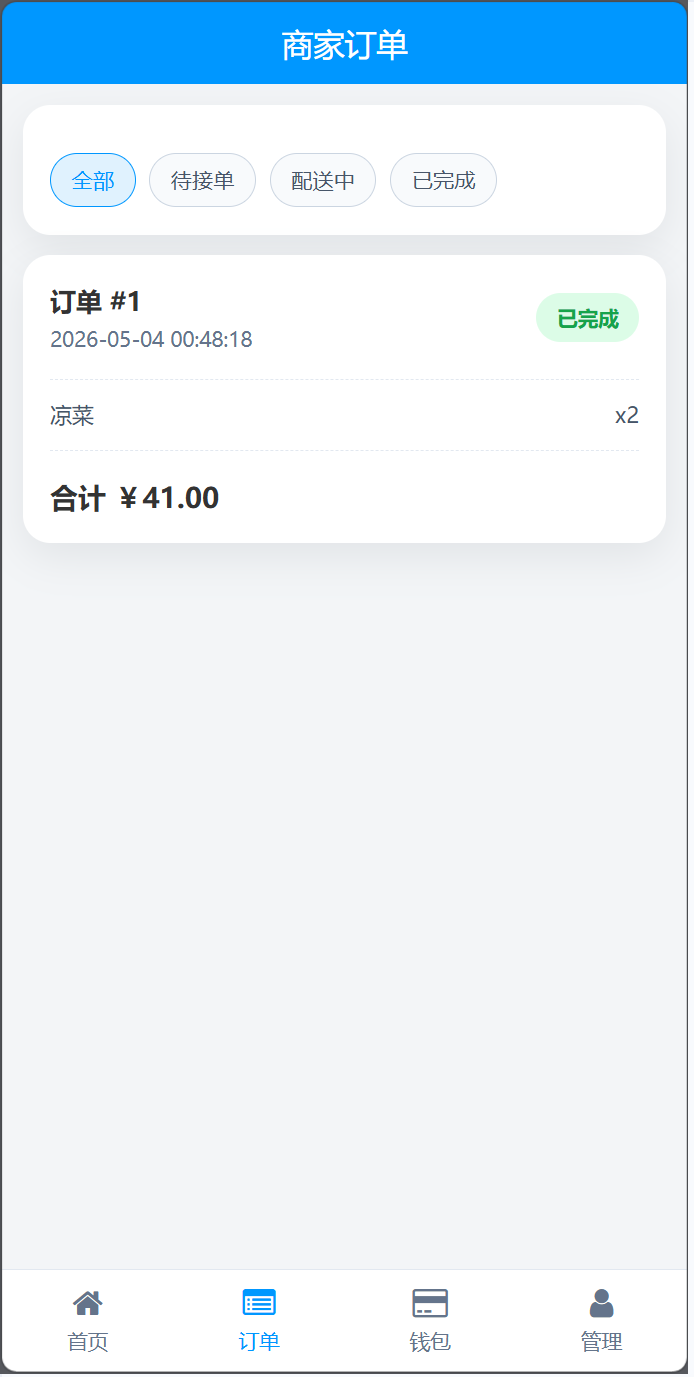
\includegraphics[width=0.75\textwidth,height=0.82\textheight,keepaspectratio]{images/page-business-orders.png}
	\caption{商家订单页面}
	\label{fig:business-orders-page}
\end{figure}

商家订单页面（BusinessOrders.vue）展示某商家收到的所有订单，支持按订单状态筛选（待支付/配送中/已送达/已完成），商家可以对订单执行确认支付、开始配送、完成配送等状态流转操作。

\section{食品与购物车模块}

\subsection{购物车页面}

\begin{figure}[H]
	\centering
	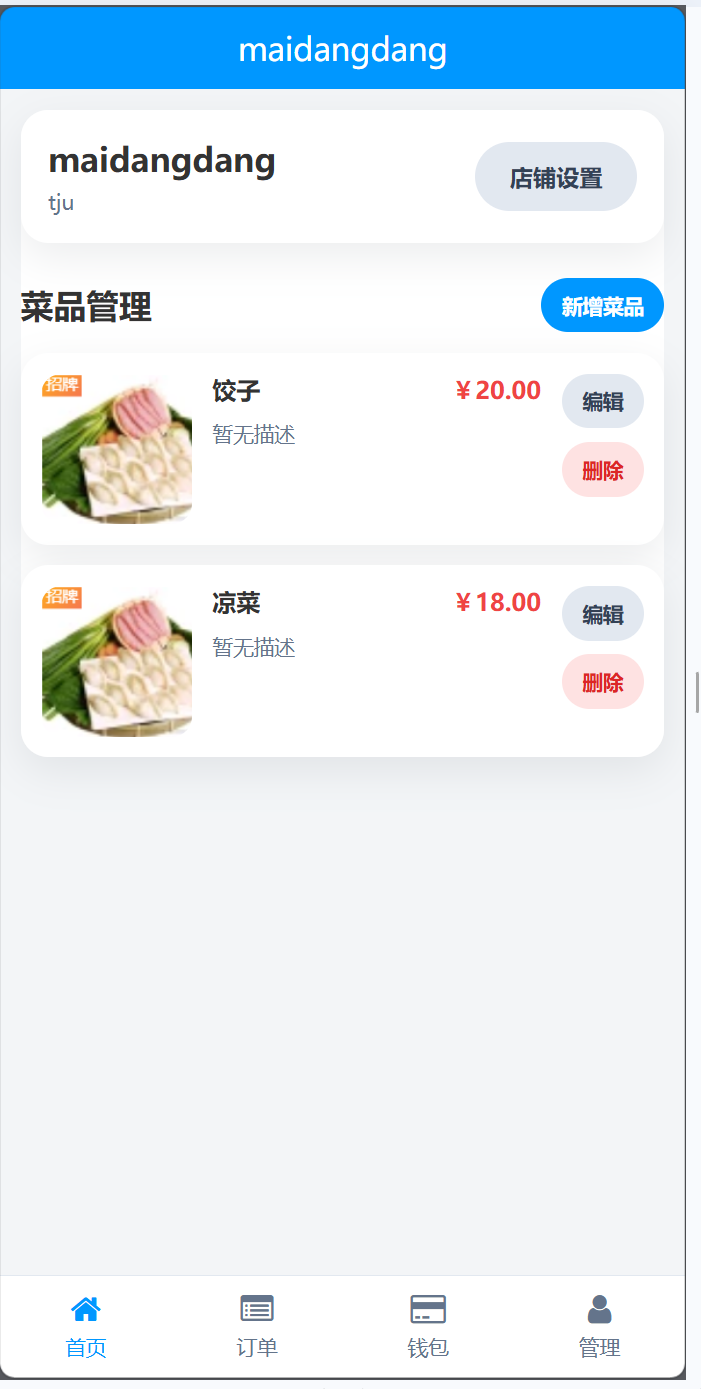
\includegraphics[width=0.75\textwidth,height=0.82\textheight,keepaspectratio]{images/page-cart.png}
	\caption{购物车页面}
	\label{fig:cart-page}
\end{figure}

购物车页面展示用户已添加的购物车项，按商家分组显示。每项显示食品名称、单价、数量和金额小计，支持修改数量和删除操作。底部合计显示总金额，提供"去结算"按钮进入下单流程。

\section{订单模块}

\subsection{订单结算页面}

\begin{figure}[H]
	\centering
	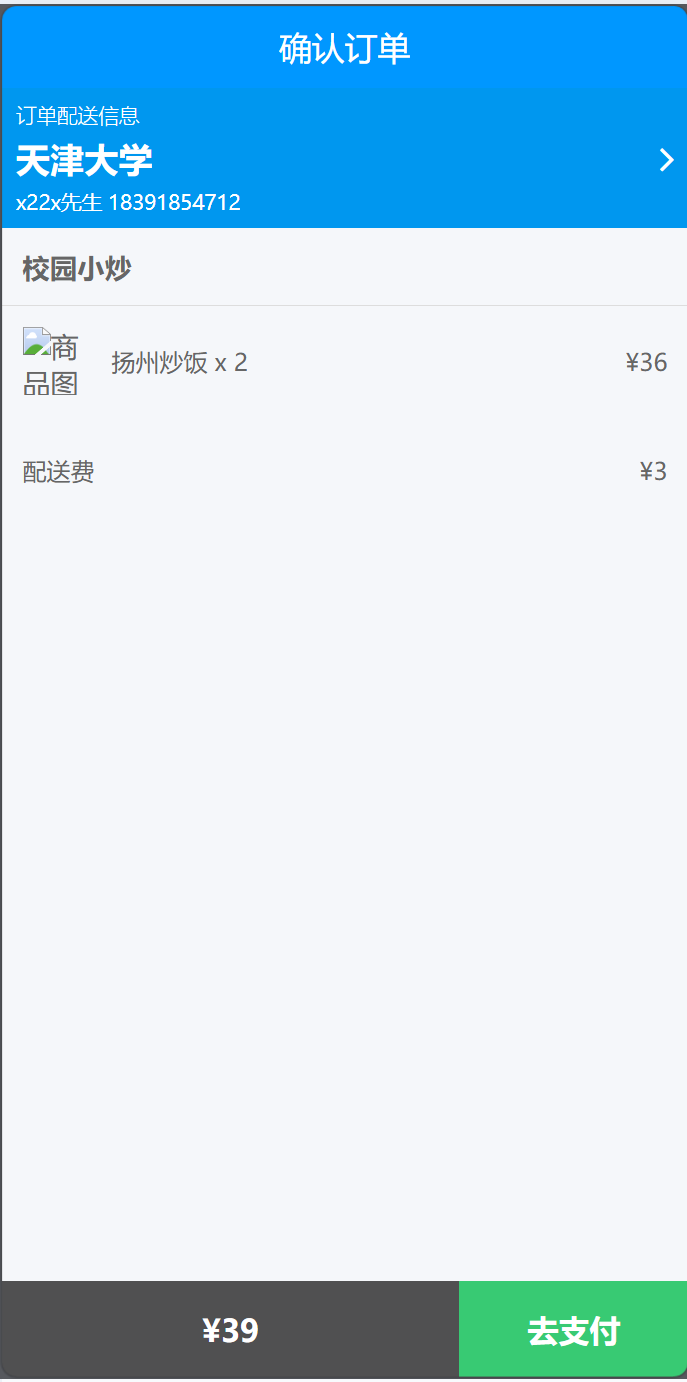
\includegraphics[width=0.75\textwidth,height=0.82\textheight,keepaspectratio]{images/page-order-checkout.png}
	\caption{订单结算页面}
	\label{fig:order-checkout-page}
\end{figure}

订单结算页面（Orders.vue）展示待提交订单的完整信息：配送地址选择、购物车商品明细、订单总金额、配送费明细。用户选择配送地址后确认下单，调用\verb|POST /orders|创建订单。

\subsection{用户订单列表页面}

\begin{figure}[H]
	\centering
	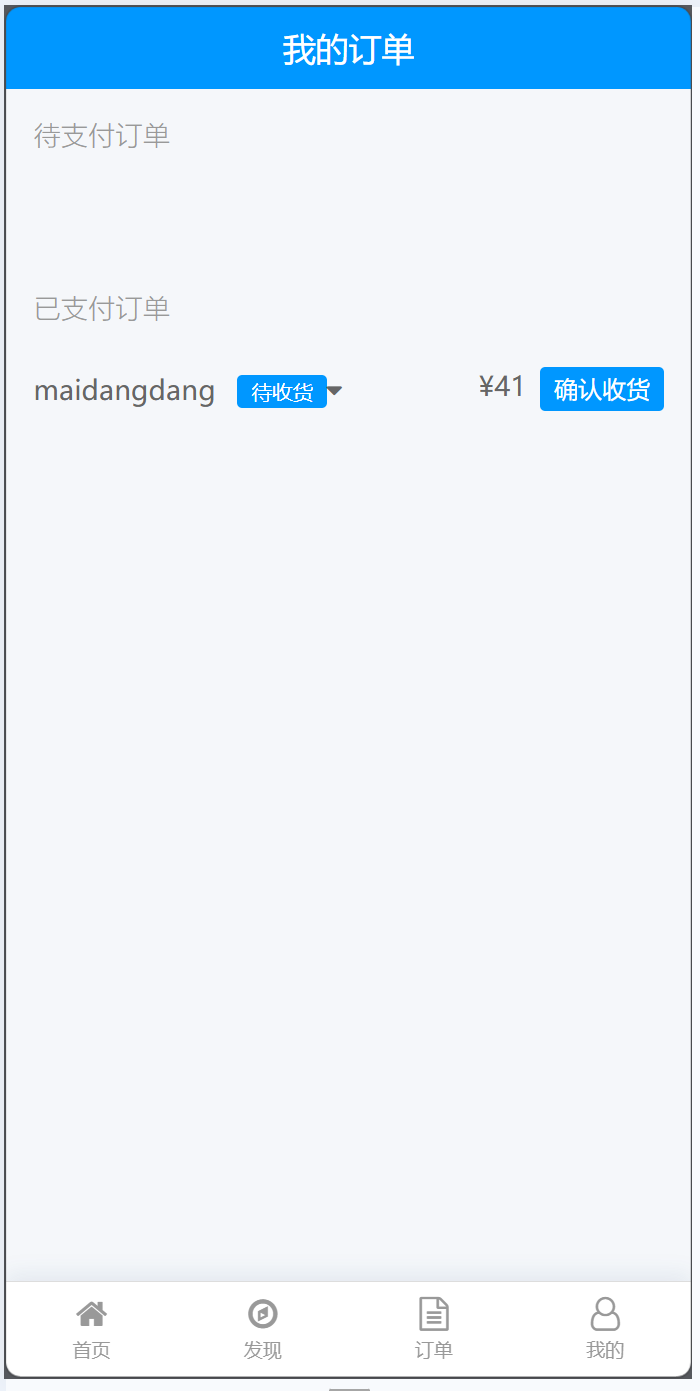
\includegraphics[width=0.75\textwidth,height=0.82\textheight,keepaspectratio]{images/page-user-order-list.png}
	\caption{用户订单列表页面}
	\label{fig:user-order-list-page}
\end{figure}

用户订单列表页面（OrderList.vue / UserOrderList.vue）展示当前用户的所有历史订单，按时间倒序排列。每个订单显示订单号、商家名称、订单总金额、订单状态（待支付/已支付/配送中/已送达/已完成）和下单时间。支持按订单状态筛选和查看订单详情。

\subsection{支付页面}

\begin{figure}[H]
	\centering
	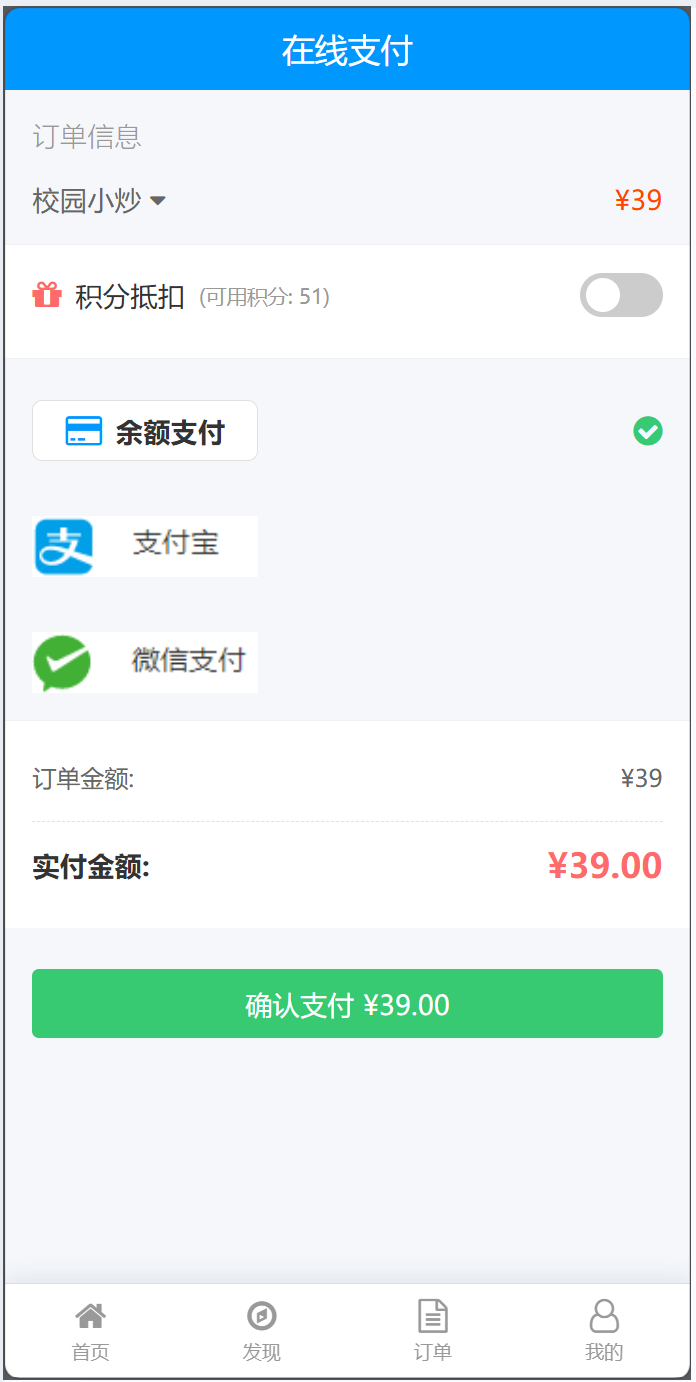
\includegraphics[width=0.75\textwidth,height=0.82\textheight,keepaspectratio]{images/page-payment.png}
	\caption{支付页面}
	\label{fig:payment-page}
\end{figure}

支付页面（Payment.vue）展示待支付订单的金额明细，支持虚拟钱包支付方式。用户确认支付后调用\verb|POST /orders/{id}/pay/virtual-wallet|，系统通过分布式锁保障交易一致性，扣除钱包余额并应用积分抵扣，更新订单状态为已支付。

\section{配送地址模块}

\subsection{地址管理页面}

\begin{figure}[H]
	\centering
	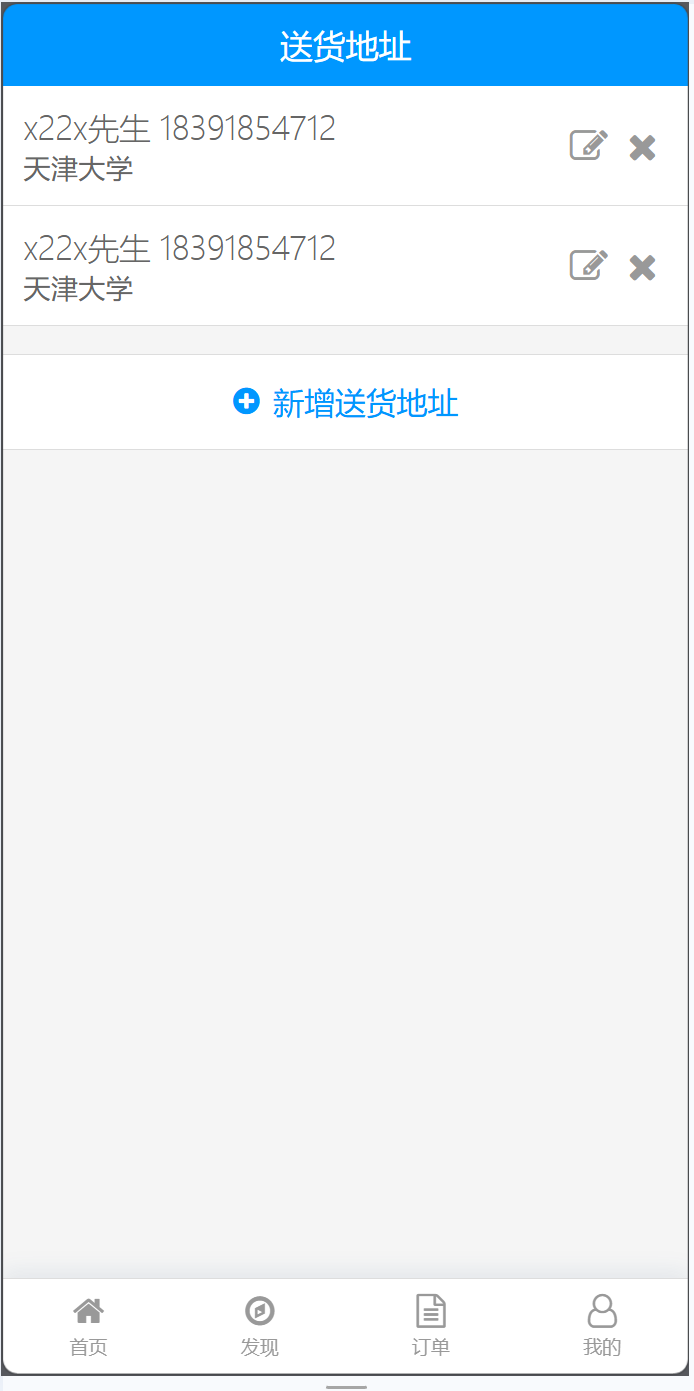
\includegraphics[width=0.75\textwidth,height=0.82\textheight,keepaspectratio]{images/page-user-address.png}
	\caption{地址管理页面}
	\label{fig:user-address-page}
\end{figure}

地址管理页面（UserAddress.vue）以列表形式展示用户所有有效配送地址，每项显示联系人姓名、性别、电话和详细地址。支持设为默认地址、编辑和删除操作。

\subsection{新增地址页面}

\begin{figure}[H]
	\centering
	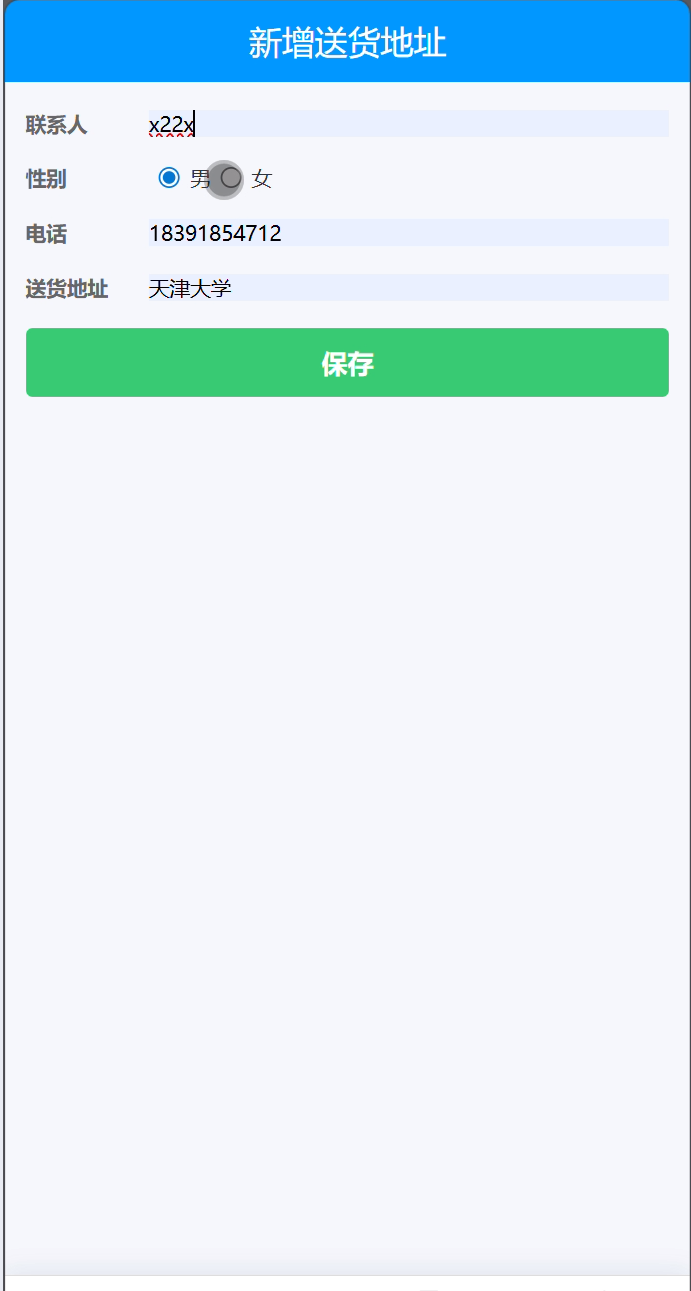
\includegraphics[width=0.75\textwidth,height=0.82\textheight,keepaspectratio]{images/page-add-address.png}
	\caption{新增地址页面}
	\label{fig:add-address-page}
\end{figure}

新增地址页面（AddUserAddress.vue）提供配送地址表单，包含联系人姓名、性别（单选）、联系电话、详细地址等字段。提交至\verb|POST /delivery-addresses|。

\subsection{编辑地址页面}

\begin{figure}[H]
	\centering
	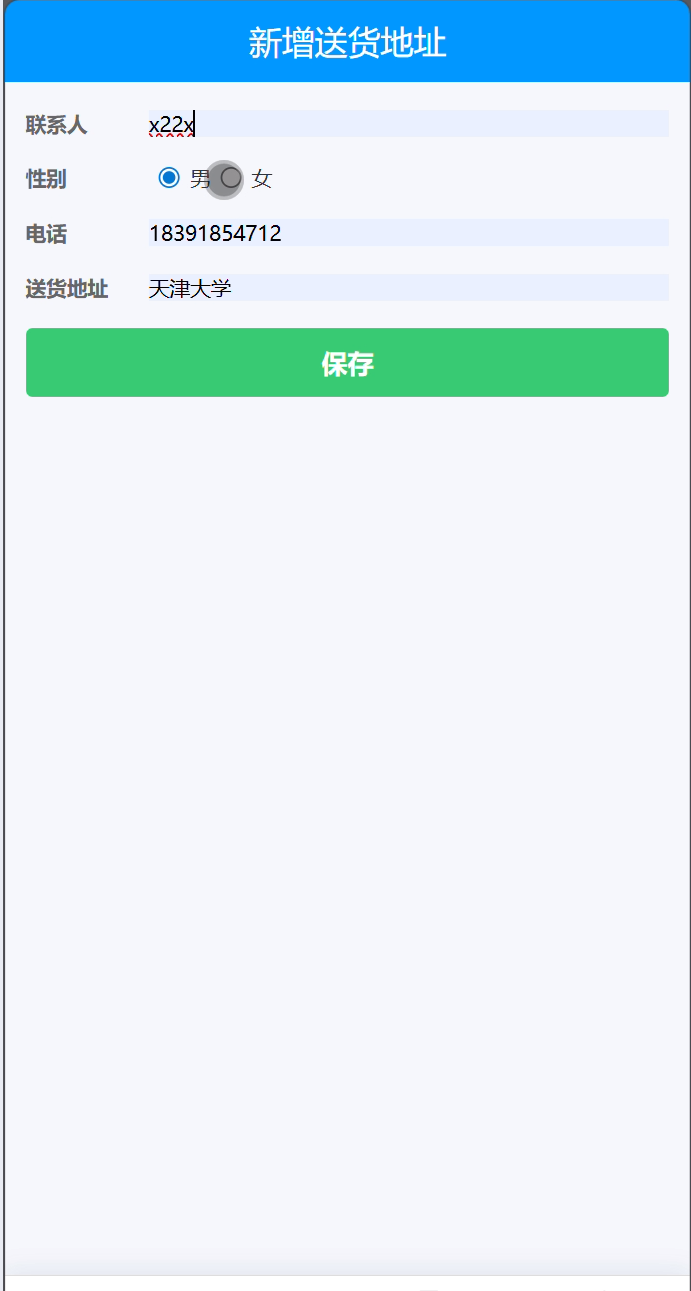
\includegraphics[width=0.75\textwidth,height=0.82\textheight,keepaspectratio]{images/page-edit-address.png}
	\caption{编辑地址页面}
	\label{fig:edit-address-page}
\end{figure}

编辑地址页面（EditUserAddress.vue）复用新增地址的表单结构，预填已有地址信息，修改后提交至\verb|PUT /delivery-addresses/{id}|。

\section{钱包模块}

\subsection{钱包页面}

\begin{figure}[H]
	\centering
	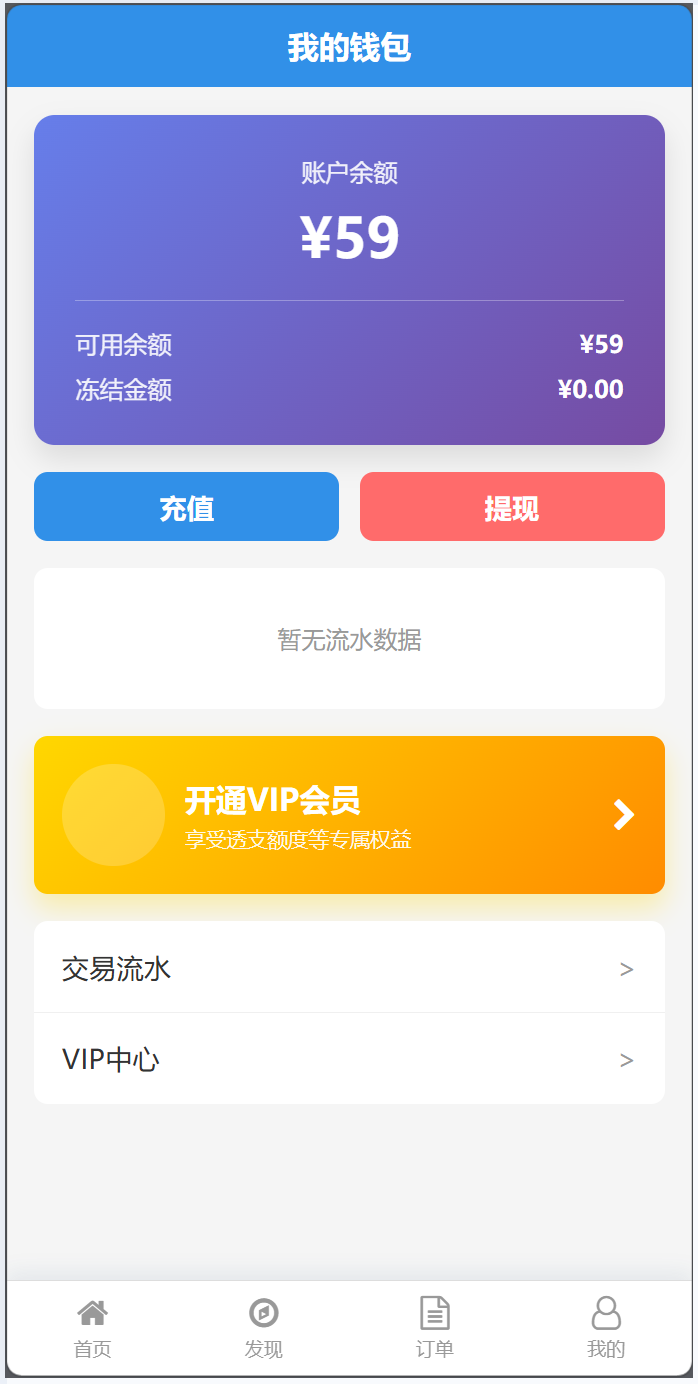
\includegraphics[width=0.75\textwidth,height=0.82\textheight,keepaspectratio]{images/page-wallet.png}
	\caption{钱包页面}
	\label{fig:wallet-page}
\end{figure}

钱包页面（Wallet.vue）展示用户虚拟钱包概览：当前余额（元）、信用额度、已用信用额度。下方提供充值、转账、提现、还款等操作入口。钱包交易的核心操作（充值、支付、转账）均受Redisson分布式锁保护。

\subsection{钱包充值页面}

\begin{figure}[H]
	\centering
	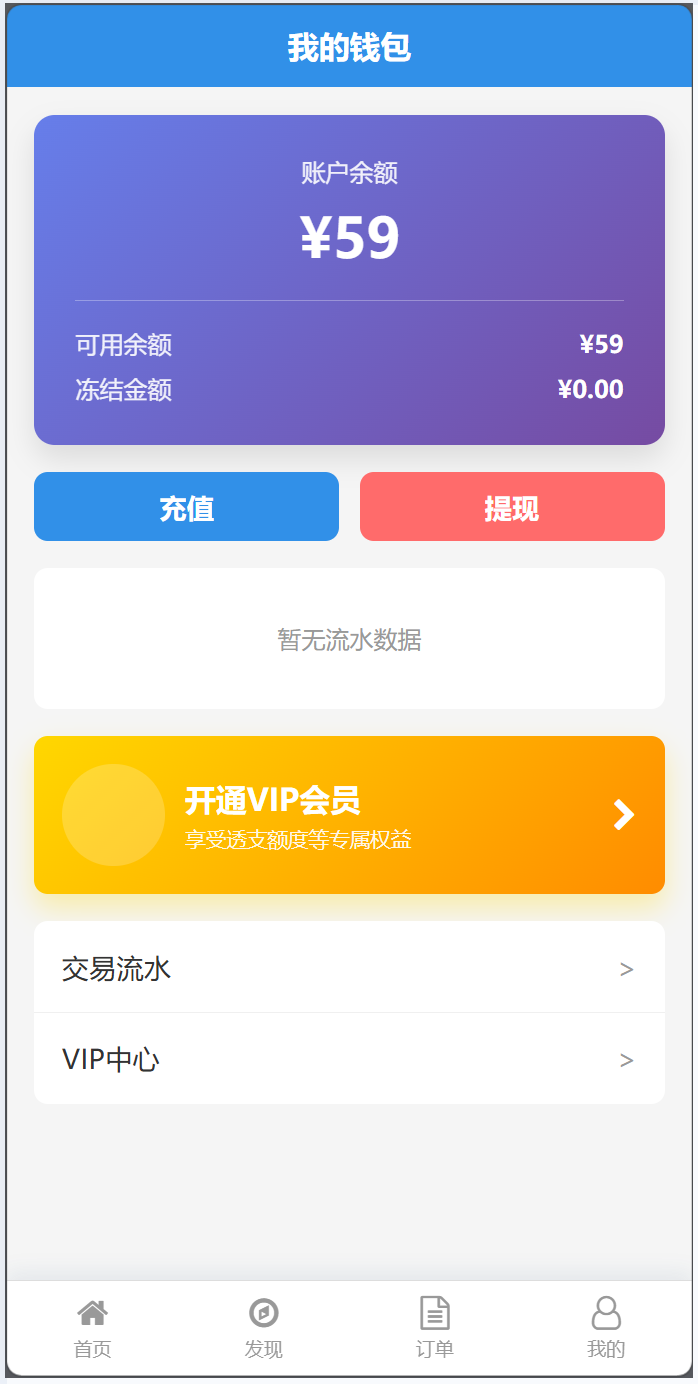
\includegraphics[width=0.75\textwidth,height=0.82\textheight,keepaspectratio]{images/page-wallet-recharge.png}
	\caption{钱包充值页面}
	\label{fig:wallet-recharge-page}
\end{figure}

钱包充值页面（WalletRecharge.vue）提供充值金额输入和支付方式选择，提交至\verb|POST /wallet/recharge|增加钱包余额。

\subsection{钱包提现页面}

\begin{figure}[H]
	\centering
	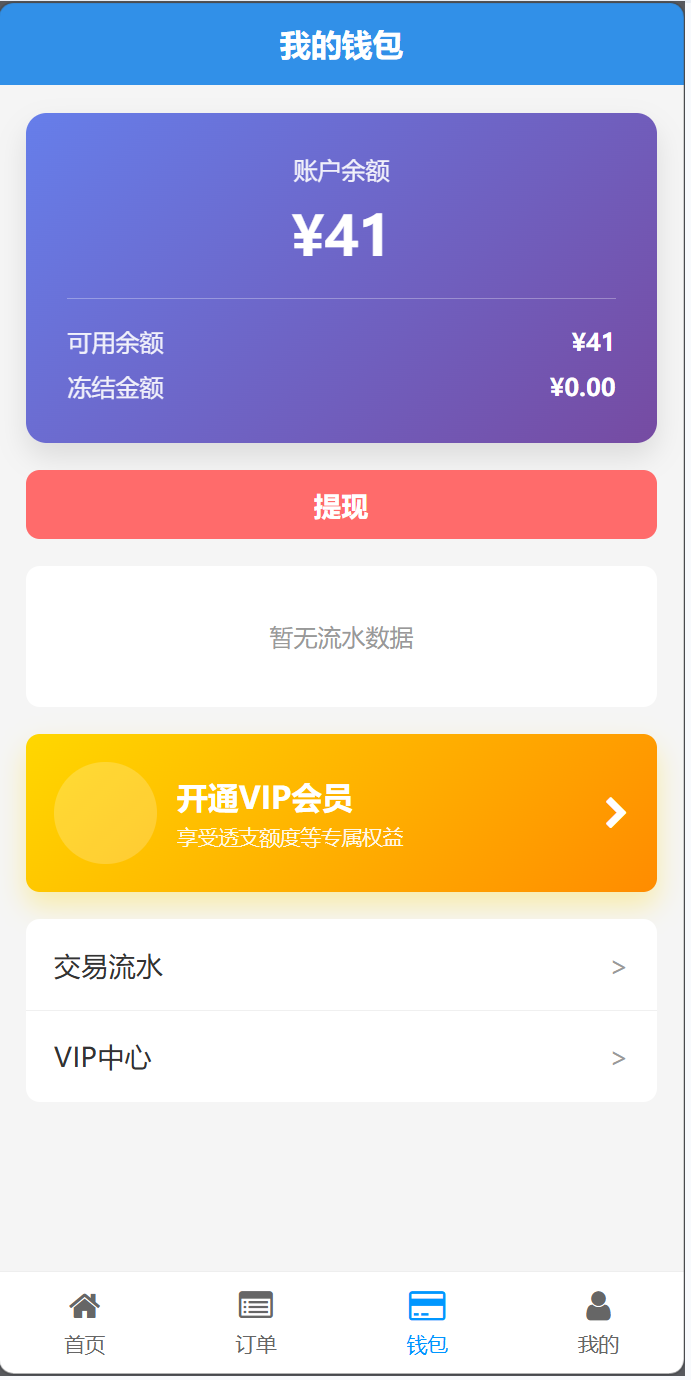
\includegraphics[width=0.75\textwidth,height=0.82\textheight,keepaspectratio]{images/page-wallet-withdraw.png}
	\caption{钱包提现页面}
	\label{fig:wallet-withdraw-page}
\end{figure}

钱包提现页面（WalletWithdraw.vue）允许用户将钱包余额提现至绑定的银行账户或支付平台。


\section{积分模块}

\subsection{积分概览页面}

\begin{figure}[H]
	\centering
	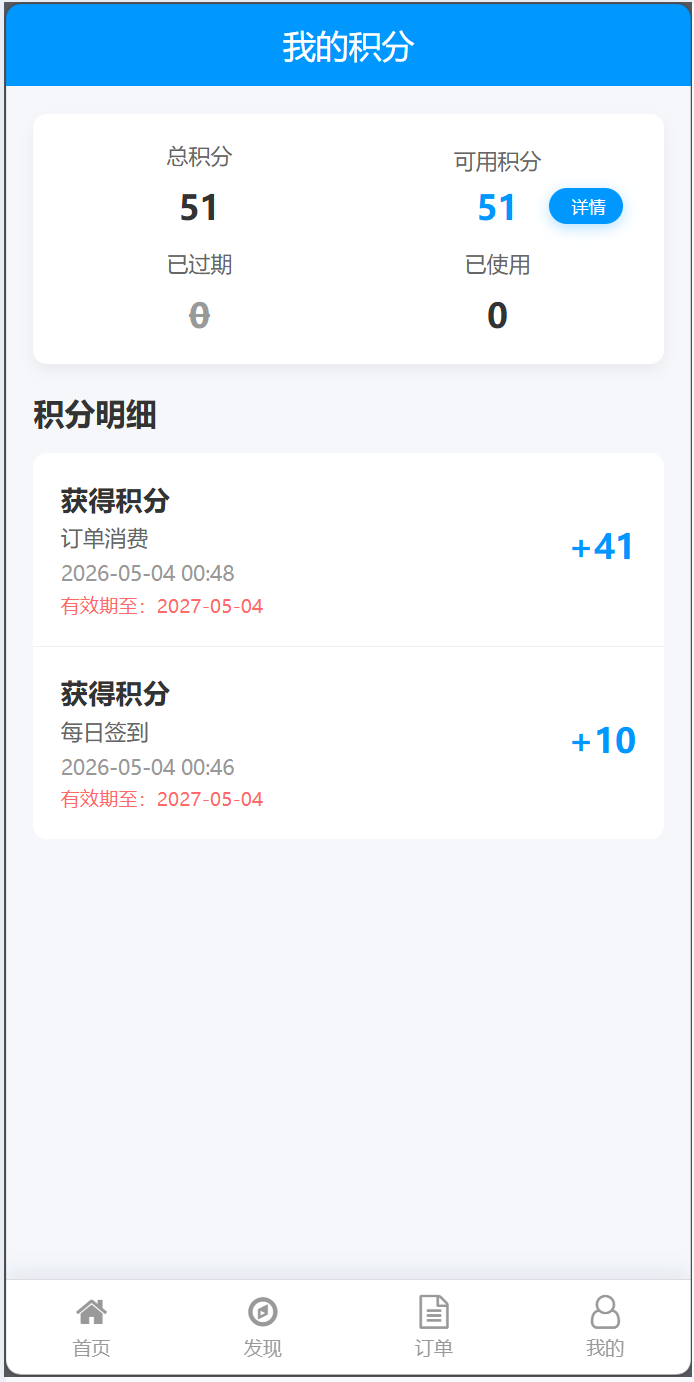
\includegraphics[width=0.75\textwidth,height=0.82\textheight,keepaspectratio]{images/page-points.png}
	\caption{积分概览页面}
	\label{fig:points-page}
\end{figure}

积分概览页面（Points.vue）展示用户积分统计信息：总积分、可用积分、已用积分、即将过期积分。下方提供签到、积分商城、积分明细等快捷入口。

\subsection{每日签到页面}

\begin{figure}[H]
	\centering
	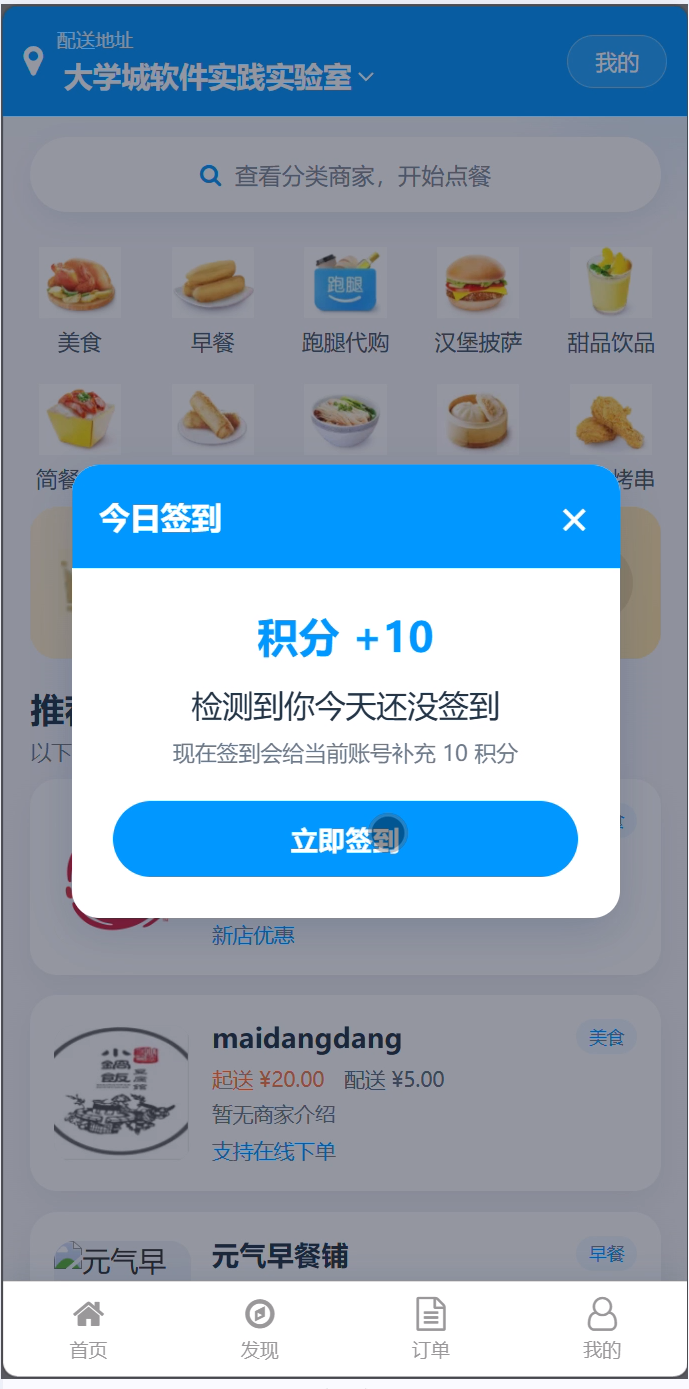
\includegraphics[width=0.75\textwidth,height=0.82\textheight,keepaspectratio]{images/page-signin.png}
	\caption{每日签到页面}
	\label{fig:signin-page}
\end{figure}

签到功能嵌入积分页面，用户每日点击签到按钮调用\verb|POST /integral/signIn|。前端展示连续签到天数和当日获得的积分奖励。连续签到天数越多，单日奖励越高，激励用户保持活跃。

\subsection{积分商城页面}

\begin{figure}[H]
	\centering
	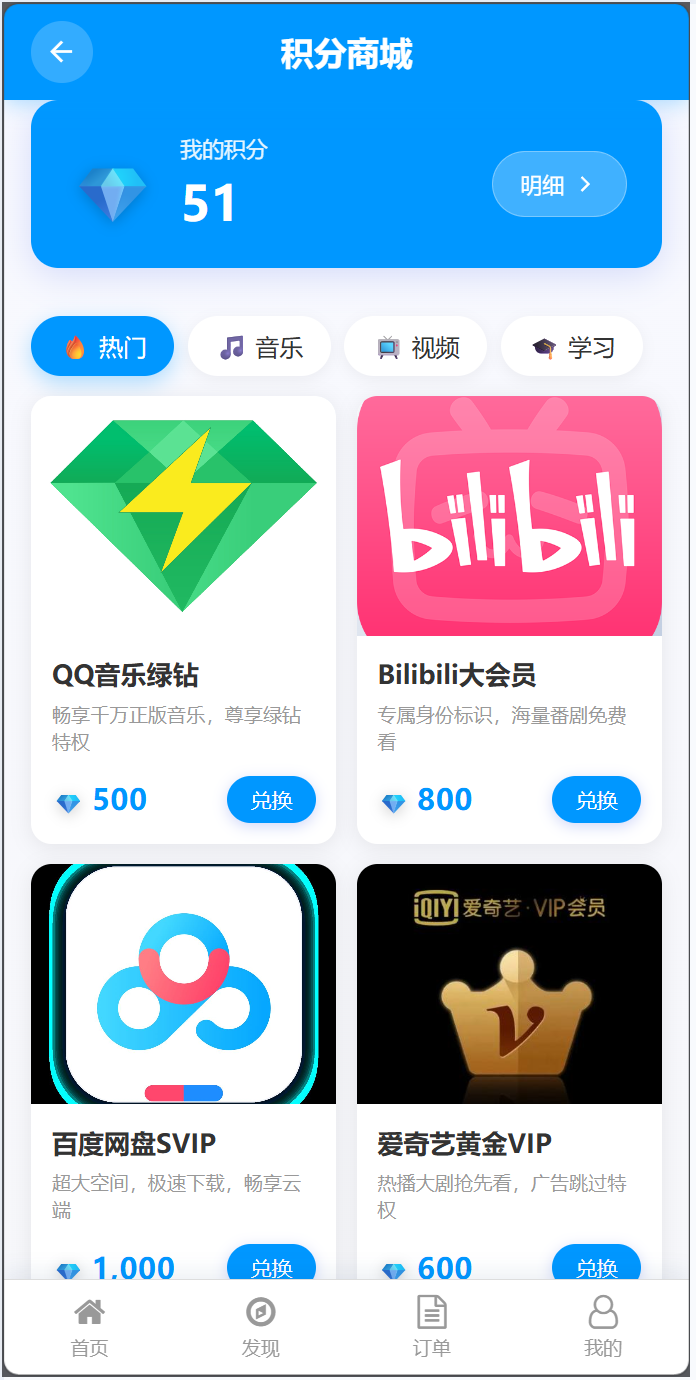
\includegraphics[width=0.75\textwidth,height=0.82\textheight,keepaspectratio]{images/page-points-mall.png}
	\caption{积分商城页面}
	\label{fig:points-mall-page}
\end{figure}

积分商城页面（PointsMall.vue）展示可使用积分兑换的商品列表（如优惠券、代金券等），每项商品显示所需积分和库存数量。用户点击兑换调用\verb|POST /integral/exchange|，扣除积分并生成兑换记录。


\section{管理员模块}

\subsection{管理员登录页面}

\begin{figure}[H]
	\centering
	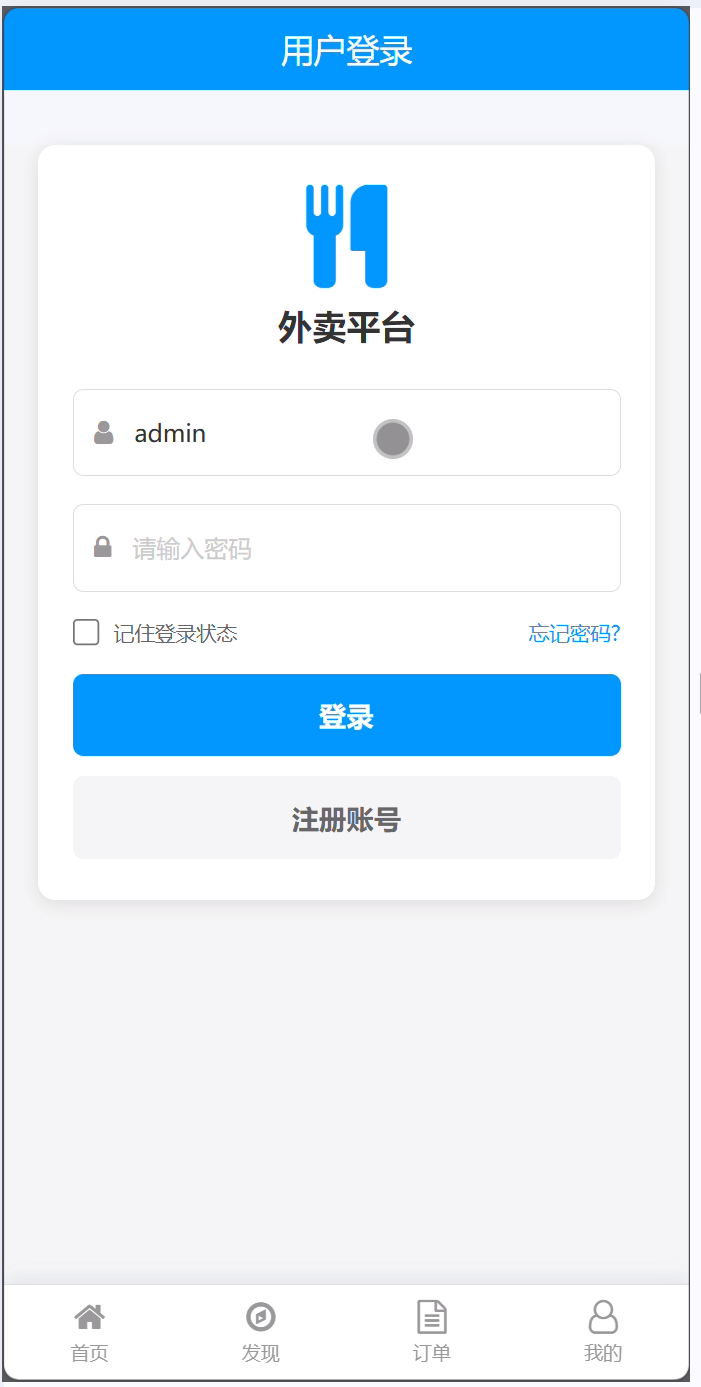
\includegraphics[width=0.75\textwidth,height=0.82\textheight,keepaspectratio]{images/page-admin-login.png}
	\caption{管理员登录页面}
	\label{fig:admin-login-page}
\end{figure}

管理员登录页面（AdminLogin.vue）提供管理员专属登录入口，与普通用户登录隔离，使用独立的管理员认证逻辑。

\subsection{用户管理页面}

\begin{figure}[H]
	\centering
	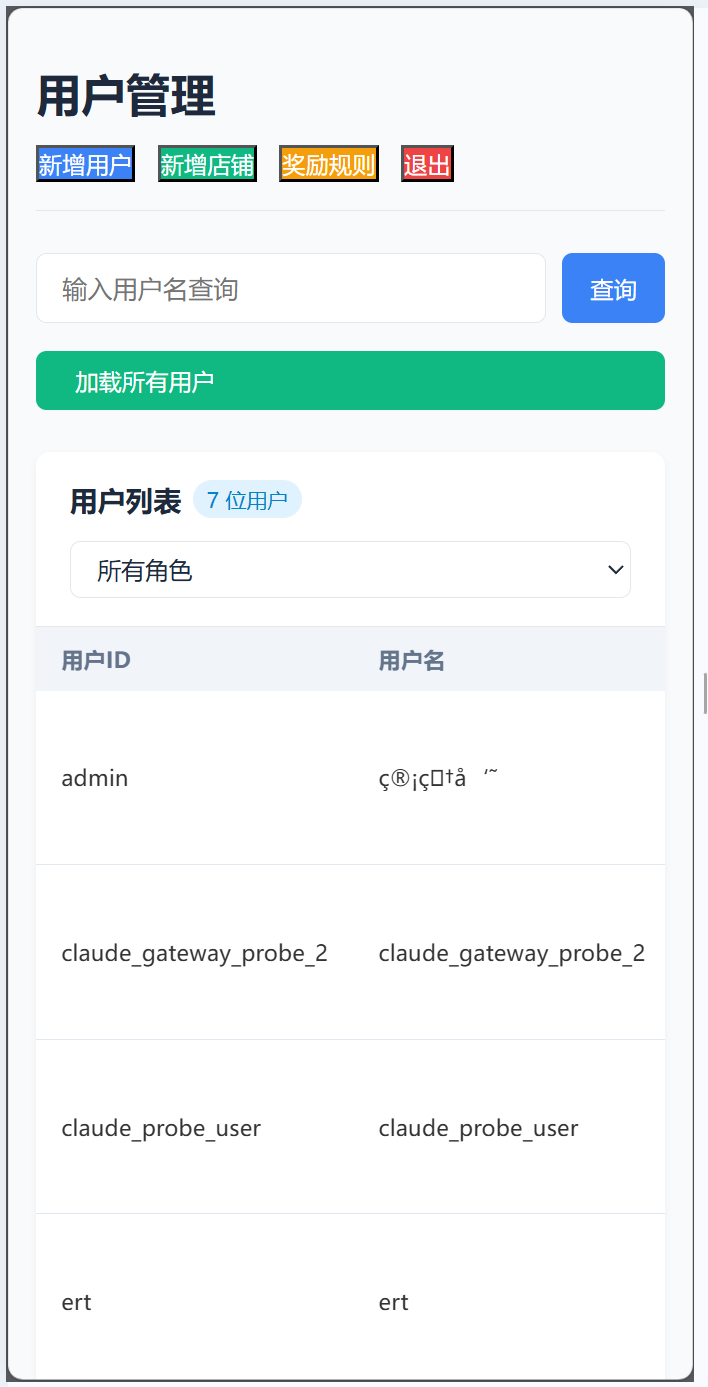
\includegraphics[width=0.75\textwidth,height=0.82\textheight,keepaspectratio]{images/page-user-management.png}
	\caption{用户管理页面}
	\label{fig:user-management-page}
\end{figure}

用户管理页面（UserManagement.vue）以表格形式展示系统所有注册用户，支持按用户名搜索、查看用户详情、启用/禁用用户账号等操作。

\subsection{添加用户页面}

\begin{figure}[H]
	\centering
	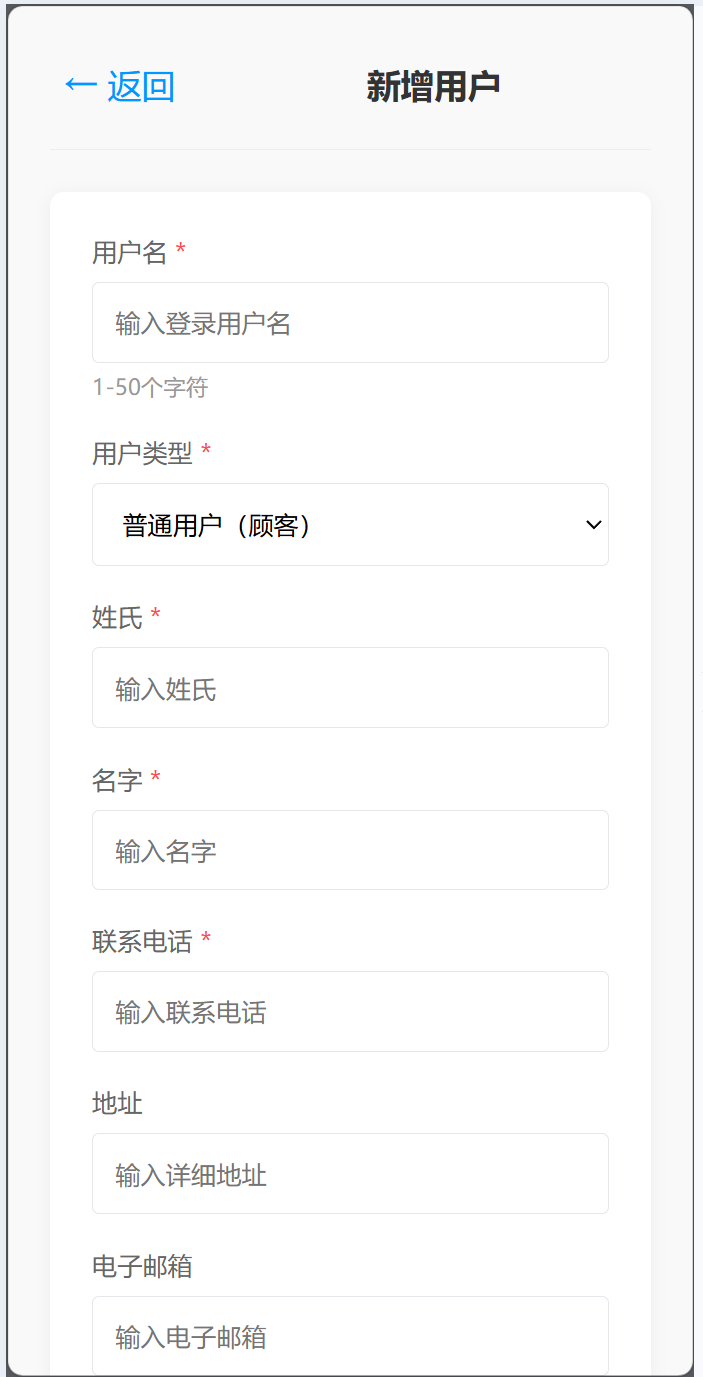
\includegraphics[width=0.75\textwidth,height=0.82\textheight,keepaspectratio]{images/page-add-user.png}
	\caption{添加用户页面}
	\label{fig:add-user-page}
\end{figure}

添加用户页面（AddUser.vue）允许管理员直接创建新用户账号，设置初始密码和基本信息。

\section{用户信息模块}

\subsection{用户信息页面}

\begin{figure}[H]
	\centering
	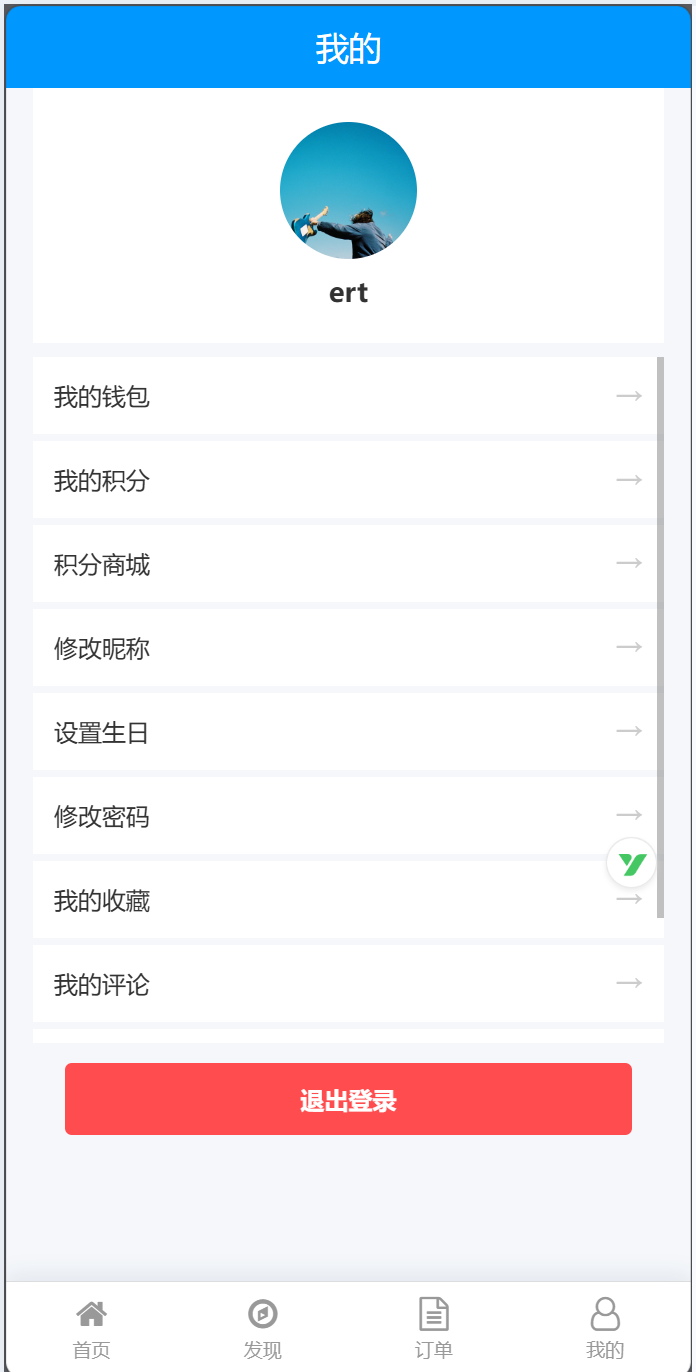
\includegraphics[width=0.75\textwidth,height=0.82\textheight,keepaspectratio]{images/page-user-info.png}
	\caption{用户信息页面}
	\label{fig:user-info-page}
\end{figure}

用户信息页面（UserInfo.vue）展示和编辑当前用户的个人资料，包括用户名、头像、性别、注册时间等。支持修改头像（上传图片）和更新基本信息。

\section{前端技术实现要点}

前端项目在技术实现上具有以下特点：

\begin{itemize}
	\item \textbf{路由管理}：使用Vue Router实现SPA路由，配置路由守卫（beforeEach）检查登录状态，未登录用户访问需认证页面时自动跳转至登录页
	\item \textbf{HTTP通信}：使用Axios封装统一的HTTP客户端，配置请求拦截器自动附加JWT Token，配置响应拦截器统一处理错误（如401未授权跳转登录页）
	\item \textbf{状态管理}：使用Vuex管理全局状态（用户信息、购物车数量徽标等）
	\item \textbf{UI组件}：使用Element Plus组件库（el-table、el-form、el-dialog、el-card等）构建统一风格的用户界面
	\item \textbf{数据可视化}：使用ECharts实现积分趋势图表、消费统计饼图等数据可视化展示
	\item \textbf{响应式布局}：使用Flex布局和Element Plus的Layout组件实现PC端和移动端的适配
	\item \textbf{容错提示}：集成GlobalFallbackRetryPrompt组件，在检测到后端服务降级响应时向用户展示友好的提示信息和重试选项
\end{itemize}

